\PassOptionsToPackage{ukrainian,english}{babel}
\documentclass[twocolumn]{el-author}

%\usepackage[...]{...}      This has been commented out as we are not using any additional packages here.  On the whole, they should be unnecessary.
\usepackage{mathtext}
\usepackage[T1,T2A]{fontenc}
\usepackage[english,ukrainian]{babel}
\usepackage{hyperref}
\usepackage{graphicx} %package to manage images
\usepackage[a4paper, total={7in, 9.5in}]{geometry}
\usepackage{makecell}
\graphicspath{ {images/} }
\newcommand{\hH}{\hat{H}}
\newcommand{\D}{^\dagger}
\newcommand{\ua}{\uparrow}
\newcommand{\nc}{\newcommand}
\renewcommand\theadfont{\normalsize\scshape}
\nc{\da}{\downarrow} \nc{\hc}{\hat{c}} \nc{\hS}{\hat{S}}
\nc{\bra}{\langle} \nc{\ket}{\rangle} \nc{\eq}{equation (\ref}
\nc{\h}{\hat} \nc{\hT}{\h{T}}\nc{\be}{\begin{eqnarray}}
\nc{\ee}{\end{eqnarray}}\nc{\rd}{\textrm{d}}\nc{\e}{eqnarray}\nc{\hR}{\hat{R}}\nc{\Tr}{\mathrm{Tr}}
\nc{\tS}{\tilde{S}}\nc{\tr}{\mathrm{tr}}\nc{\8}{\infty}\nc{\lgs}{\bra\ua,\phi|}\nc{\rgs}{|\ua,\phi\ket}
\nc{\hU}{\hat{U}}\nc{\lfs}{\bra\phi|}\nc{\rfs}{|\phi\ket}\nc{\hZ}{\hat{Z}}\nc{\hd}{\hat{d}}\nc{\mD}{\mathcal{D}}
\nc{\bd}{\bar{d}}\nc{\bc}{\bar{c}}\nc{\mc}{\mathcal}\nc{\ea}{eqnarray}\nc{\mG}{\mathcal{G}}\nc{\bce}{\begin{center}}
\nc{\ece}{\end{center}}
\date{20 Грудня 2018}

\begin{document}

\title{Назва}

\author{Сергій Поліщук}

\abstract{Абстакція}

\maketitle

\section{Мета роботи}

Тут мета

\section{Прилади і матеріали}

Тут Прилади і мателіали

\section{Завдання}

\begin{enumerate}
	\item при домашній підготовці:
	\begin{itemize}
		\item  
		\item  
		\item  
	\end{itemize}
	\item при виконанні роботи:
	\begin{itemize}
		\item  
		\item  
		\item  
		\item  
		\item  
	\end{itemize}
	
\end{enumerate}

\section{Правила техніки безпеки}

\begin{itemize}
	\item  
	\item  
	\item  
\end{itemize}

\section{Теоретичні відомості та опис установки}



%\begin{equation} \label{eq:Einstein}
%hv = A+\frac{m_{e}V_{max}^{2}}{2}
%\end{equation}

%\begin{figure}[h]
%\centering{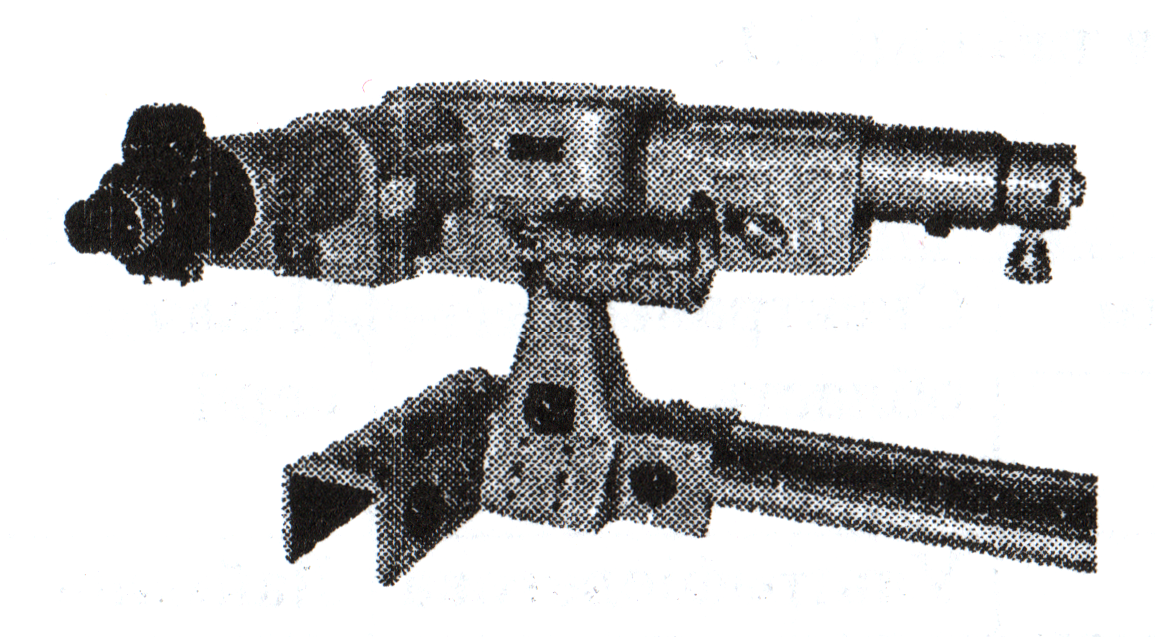
\includegraphics[width=80mm]{img_1}}
%\caption{\source{}}
%\label{img:1}
%\end{figure}

%\begin{table}[ht]
%\processtable{Спектральні характеристики деяких скляних світлофільтрів}
%{\begin{tabular}{|l|l|l|l|l|}\hline
%\thead{№} & 
%\thead{{\scriptsize Марка} \\ {\scriptsize світлофільтра}} & 
%\thead{{\scriptsize Товщина} \\ {\scriptsize скла, мм}} & 
%\thead{{\scriptsize Довжина хвилі} \\ {\scriptsize максимального} \\ {\scriptsize пропускання, м}} & 
%\thead{{\scriptsize Частота хвилі} \\ {\scriptsize максимального} \\ {\scriptsize пропускання, Гц}}\\\hline
%1 & КС-13 & 2,78 & $700*10^{-9}$ & $4.3*10^{14}$ \\\hline
%2 & OC-13 & 3,02 & $650*10^{-9}$ & $4.6*10^{14}$ \\\hline
%3 & ЖС-18 & 3,07 & $600*10^{-9}$ & $5.0*10^{14}$ \\\hline
%4 & 3C-1 & 1,00 & $540*10^{-9}$ & $506*10^{14}$ \\\hline
%5 & CC-2 & 1,00 & $390*10^{-9}$ & $7.7*10^{14}$ \\\hline
%6 & ФС-6 & 1,00 & $360*10^{-9}$ & $8.3*10^{14}$ \\\hline
%\end{tabular}}{}
%\end{table}


\section{Послідовність виконання роботи}

\begin{thebibliography}{}

\bibitem{1}
Кучерук І.М., Горбачук І.Т. Загальний курс фізики: Т.3.: Оптика.
Квантова фізика. - К.: Техніка, 2006.- 518c., cr. 239 - 247.

\bibitem{2}
Кучерук ІМ, Дущенко В.П. Загальна фізика. Оптика. Квантова
фізика. - К.: Вища школа, 1999. -- 463с., ст. 260 - 264.

\bibitem{3}
орбачук ІТ. Загальна фізика. Лабораторний практикум. - К.:
Вища школа, 1992.- 512 с., ст. 434 - 437.

\bibitem{4}
Методична розробка до роботи.

\end{thebibliography}

\section{Завдання для самоконтролю}

\begin{enumerate}
	\item 
	\item 
	\item 
	\item 
	\item 
	\item 
	\item 
	\item 
	\item 
	\item 
	\item 
	\item 
	\item 
	\item 
	\item 
\end{enumerate}

\clearpage
\section{Тестові завдання для вхідного контролю}

\begin{enumerate}
	\item 
	\begin{enumerate}
		\item 
		\item 
		\item 
		\item 
	\end{enumerate}
	\item 
	\begin{enumerate}
		\item 
		\item 
		\item 
		\item 
	\end{enumerate}
	\item 
	\begin{enumerate}
		\item 
		\item 
		\item 
		\item 
	\end{enumerate}
	\item 
	\begin{enumerate}
		\item 
		\item 
		\item 
		\item 
	\end{enumerate}
	\item 
	\begin{enumerate}
		\item 
		\item 
		\item 
		\item 
	\end{enumerate}
	\item 
	\begin{enumerate}
		\item 
		\item 
		\item 
		\item 
	\end{enumerate}
	\item 
	\begin{enumerate}
		\item 
		\item 
		\item 
		\item 
	\end{enumerate}
\end{enumerate}

\newpage

\section{Тестові завдання для підсумкового контролю}

\begin{enumerate}
	\item 
	\begin{enumerate}
		\item 
		\item 
		\item 
		\item 
	\end{enumerate}
	\item 
	\begin{enumerate}
		\item 
		\item 
		\item 
		\item 
	\end{enumerate}
	\item 
	\begin{enumerate}
		\item 
		\item 
		\item 
		\item 
	\end{enumerate}
	\item 
	\begin{enumerate}
		\item 
		\item 
		\item 
		\item 
	\end{enumerate}
	\item 
	\begin{enumerate}
		\item 
		\item 
		\item 
		\item 
	\end{enumerate}
\end{enumerate}

\end{document}

%\begin{table}[b]
%\processtable{Coefficients and remainders for distribution KK ($k = 0.05$,
%$v = 3$, $c_{1} = 1.5$, $c_{2} = 4.5$)}
%{\begin{tabular}{|l|l|l|}\hline
%$n$ & $a_{n}^{2}$ & $r_{k}(1)$\\\hline
%0 & 3.602576748428 & 1.493719547999\\\hline
%1 & 1.384791111989 & 0.108928436101\\\hline
%2 & 0.108600438794 & 0.000327997399\\\hline
%3 & 0.000275794597 & 0.000052202814\\\hline
%4 & 0.000027616892 & 0.000024585922\\\hline
%5 & 0.000018178621 & 0.000006407300\\\hline
%\end{tabular}}{}
%\end{table}
%
%So, the basic preamble and main body will be:
%\verb"\documentclass[twocolumn]{el-author}"\\
%\verb"\usepackage[...]{packages}"\\
%\verb"\date{12 December 2012}"\\
%\verb"\title{...}"\\
%\verb"\author{...}"\\
%\verb"\abstract{...}"\\
%\verb"\maketitle{...}"\\
%\verb"\begin{document}"\\
%\verb"..."\\
%\verb"\section{...}"\\
%\verb"..."\\
%\verb"\section{..}"\\
%\verb"..."\\
%\verb"\end{document}"